% --- Dreamer, DreamerV2, DreamerV3 ---
\begin{frame}[t]{Dreamer: motivation}
    \begin{columns}
      \begin{column}{0.5\textwidth}
        \centering
        Model-based RL agent with an RSSM core that reaches state-of-the-art performance on image-based control tasks while requiring fewer samples.
      \end{column}
      \begin{column}{0.5\textwidth}
        \centering
        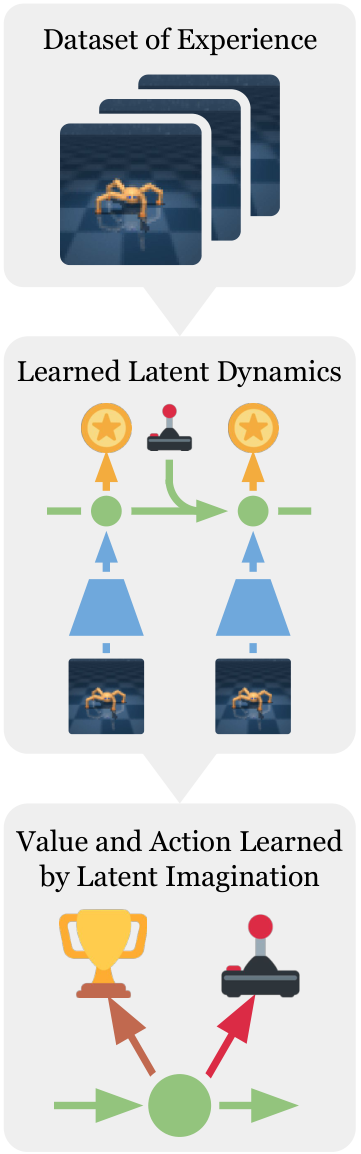
\includegraphics[width=0.95\linewidth,height=0.78\textheight,keepaspectratio]{images/world-models/towardsai_primer_dreamer_hafner2020_iclr_p1_teaser.png}\\[0.12em]
        {\scriptsize Hafner et al., \href{https://arxiv.org/pdf/1912.01603.pdf}{\textit{Dream to Control}}. Chen, \href{https://pub.towardsai.net/dreamer-8b5a42acebbf}{Towards AI} (2020).}
      \end{column}
    \end{columns}
\end{frame}

\begin{frame}[t]{Dreamer: architecture}
  \centering
  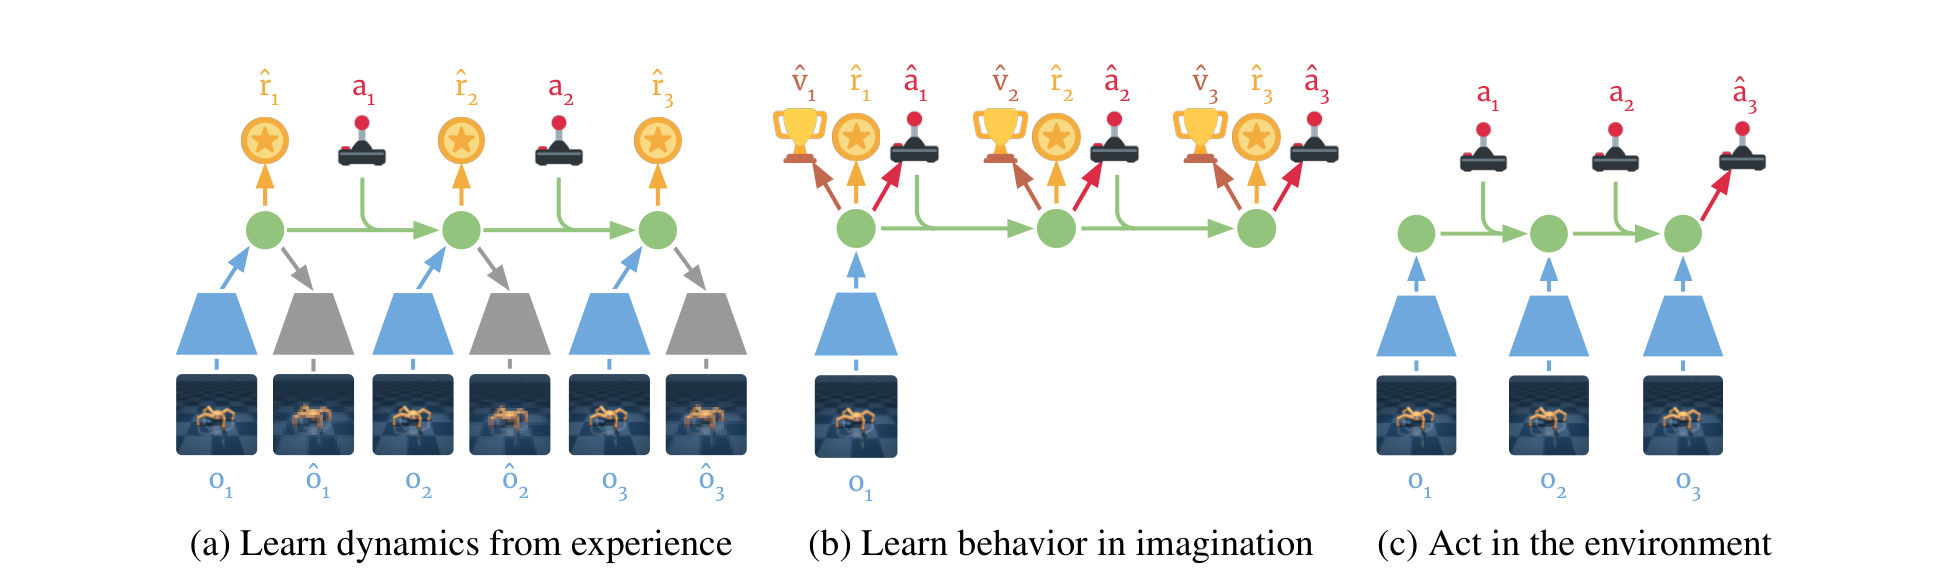
\includegraphics[width=\linewidth,height=0.84\textheight,keepaspectratio]{images/world-models/towardsai_primer_dreamer_hafner2020_iclr_fig3_components.png}
  {\tiny Dreamer architecture. Diagram credit: Hafner et al.\ (ICLR 2020), \href{https://arxiv.org/pdf/1912.01603.pdf}{PDF}}\\[0.2em]
  Dreamer is composed of three main parts:
  \begin{itemize}\itemsep0.08em \footnotesize
    \item \textbf{ (a) Dynamics Learning:} learns representation, transition, reconstruction, reward models.
    \item \textbf{ (b) Behavior Learning:} based on the dynamics model, learns actor--critic architecture to maximize rewards.  
    \item \textbf{ (c) Environment Interaction:} using action model for data collection.
  \end{itemize}
\end{frame}

% --- Behaviors learned in imagination (the PlaNet -> Dreamer pivot) ---
\begin{frame}[t]{Dreamer: Learning Behaviors in Imagination}
  \begin{itemize}\itemsep0.28em
    \item Instead of planning at act time (PlaNet), Dreamer trains an \textbf{actor} and a \textbf{critic} on \textbf{imagined latent trajectories}.
    \item Rollouts never touch pixels: start from latent states of replayed real experience, then unroll the RSSM \textbf{prior} for a short horizon.
    \item The \textbf{critic} estimates value beyond the horizon; the \textbf{actor} is improved by backpropagating value gradients \textbf{through the learned dynamics}, which is possible because the world model is differentiable.
    \item Result: acting is a single forward pass (no per-step search), and the critic gives long-horizon credit assignment that CEM planning lacked.
  \end{itemize}
\end{frame}

\begin{frame}[t]{DreamerV2: discrete world model \& V1 $\rightarrow$ V2}
  \begin{columns}
    \column{0.64\textwidth}
    \centering
    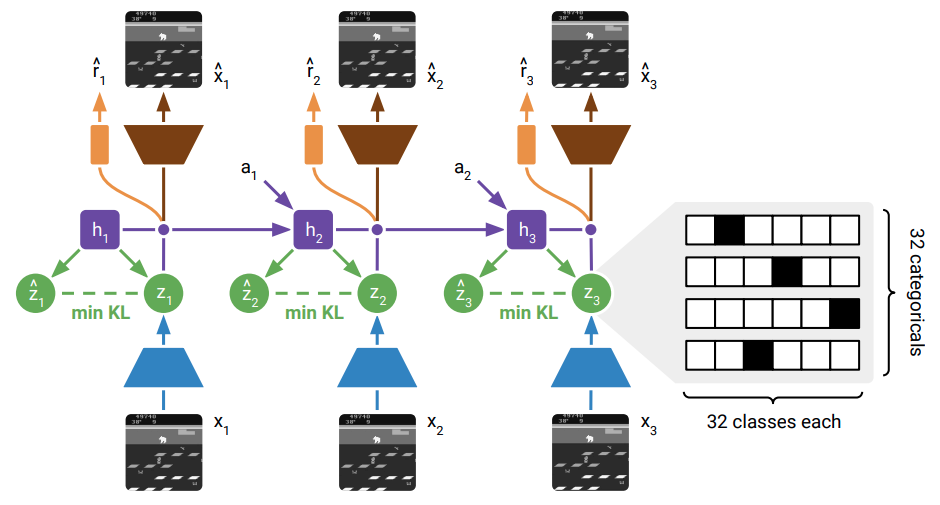
\includegraphics[width=0.94\linewidth,height=0.94\textheight,keepaspectratio]{images/world-models/eclecticsheep_dreamerv2_worldmodel_arch.png}\\[0.08em]
    {\tiny World-model overview. Diagram credit: Belotti (2023)}
    \column{0.36\textwidth}
    \begin{itemize}\footnotesize
      \item \textbf{Key upgrade:} The world model now uses \textbf{discrete categorical latents} instead of continuous Gaussian variables. Each latent consists of 32 variables, each taking one of 32 categories, enabling a richer and more expressive latent space.
      \item Discrete latents are optimized using \textbf{straight-through gradients} for effective backpropagation despite non-differentiability. This allows for more precise representation and imagination.
      \item \textbf{KL balancing} is introduced to stabilize training by balancing the KL divergence term across model components.
    \end{itemize}
  \end{columns}
\end{frame} 

\begin{frame}[t]{DreamerV3: motivation}
  \begin{itemize}\itemsep0.10em
    \item Achieves state-of-the-art performance across 150+ diverse tasks with a single configuration.
    \item Learns a world model to imagine future trajectories. Successfully solves challenging open-world environments such as collecting diamonds in Minecraft without human data.
    \item Architecturally similar to DreamerV2. Robustness and scalability stem from careful normalization, balancing, and mathematical tricks that enable stability across domains.
  \end{itemize}
\end{frame}

\begin{frame}[t]{DreamerV3: architecture}
  Learning algorithm consists of three neural networks:
  \begin{itemize}\itemsep0.06em\footnotesize
    \item \textbf{World model:} RSSM model that predicts the outcomes of potential actions, modeling future states of the environment.
    \item \textbf{Critic:} Judges the value of each predicted outcome, estimating how beneficial a state is for achieving the agent's goals.
    \item \textbf{Actor:} Selects actions intended to achieve the most valuable outcomes by maximizing the evaluated value.
  \end{itemize}
  \vspace{-0.4em}
  \centering
  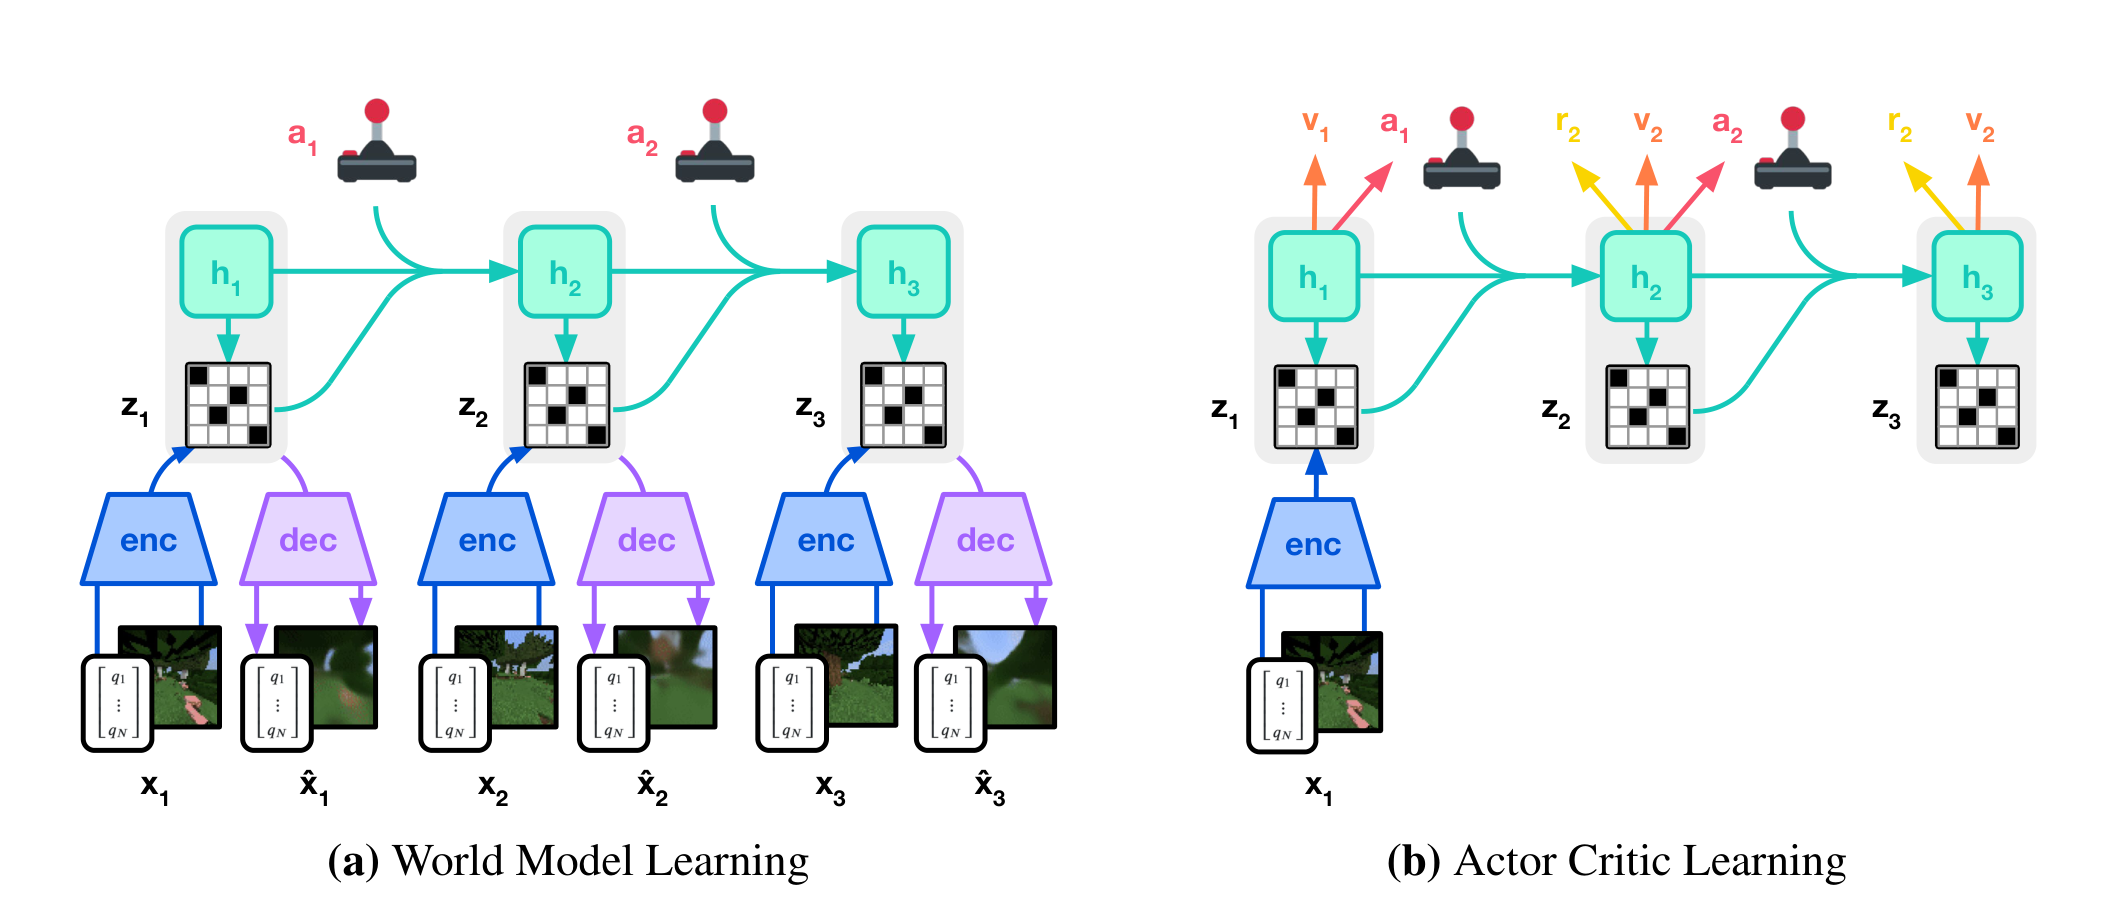
\includegraphics[width=\linewidth,height=0.46\textheight,keepaspectratio]{images/world-models/dreamerv3_arxiv2301_fig3_training_process.png}\\[0.03em]
  {\scriptsize Hafner et al., \href{https://arxiv.org/pdf/2301.04104.pdf}{arXiv:2301.04104}.}
\end{frame}

% --- What actually makes V3 stable across domains ---
\begin{frame}[t]{DreamerV3: What Makes It Stable}
  The ``mathematical tricks'' behind one configuration for 150+ tasks:
  \begin{itemize}\itemsep0.26em
    \item \textbf{Symlog predictions:} inputs and regression targets pass through a signed-log transform, taming value scales that differ by orders of magnitude across domains.
    \item \textbf{Two-hot return targets:} the critic predicts a distribution over discretized returns instead of a single scalar, which is more robust to outliers.
    \item \textbf{KL balancing and free bits:} the world-model KL term is split and clipped so neither prior nor posterior collapses, and small KL values are not over-optimized.
    \item \textbf{Percentile return normalization:} rewards are normalized by a running percentile range, so exploration behaves consistently across dense and sparse rewards.
    \item Published in \emph{Nature} (2025); the headline demo is collecting diamonds in Minecraft from scratch, without human data.
  \end{itemize}
\end{frame}

\begin{frame}[t]{DreamerV3: results}
  \centering
  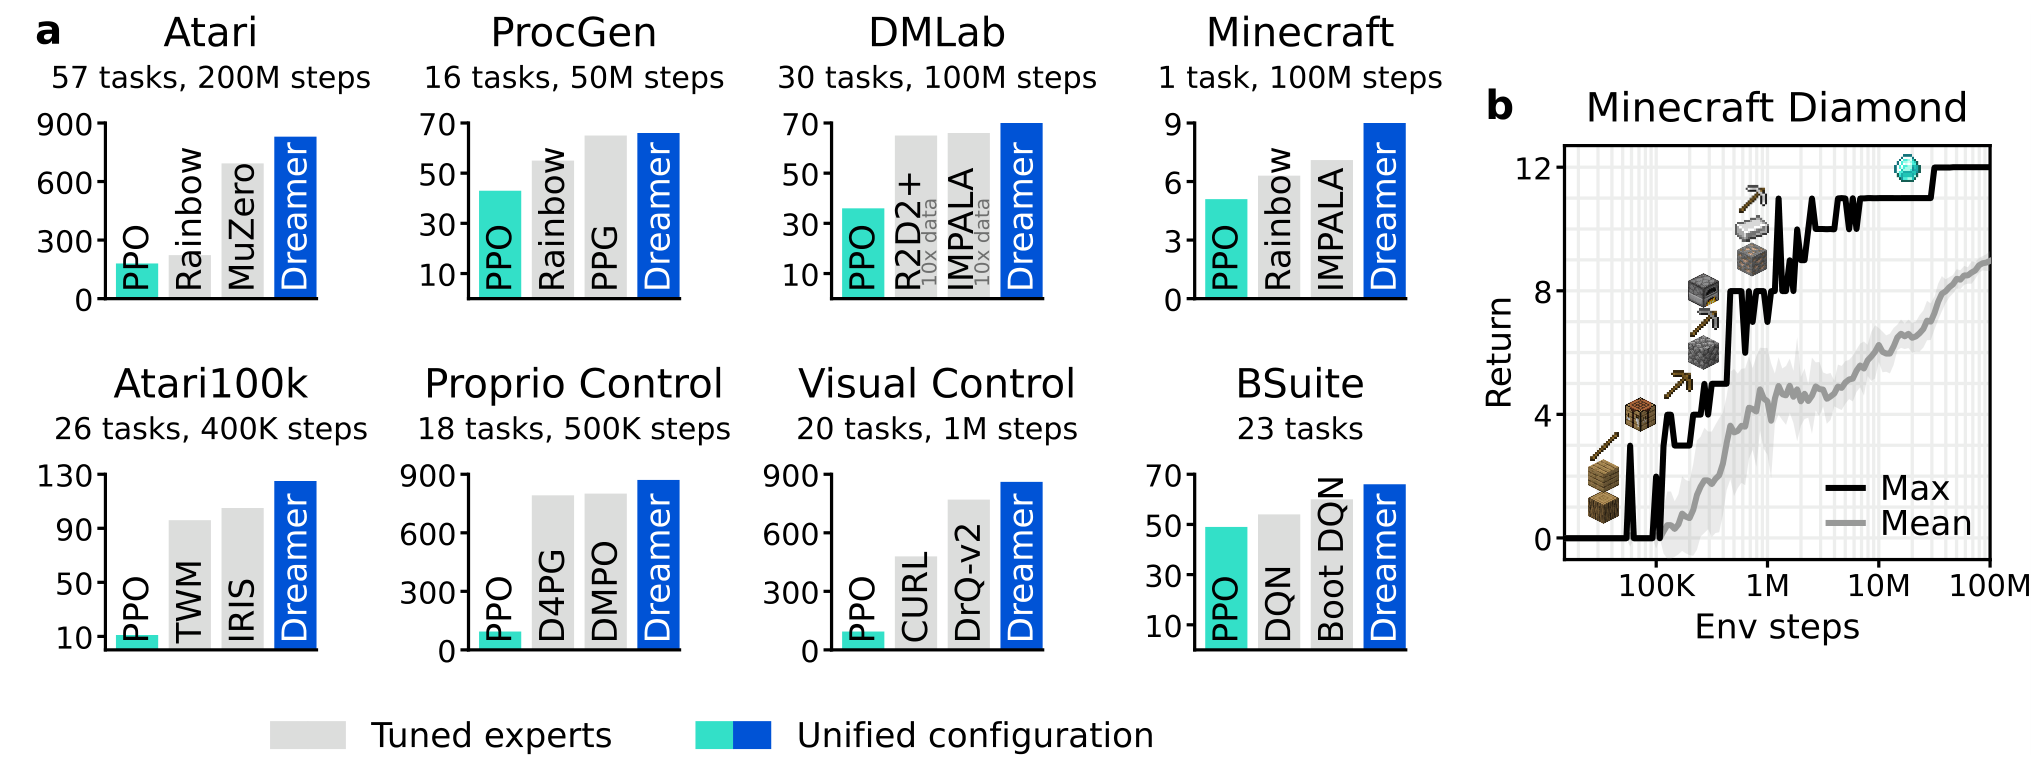
\includegraphics[width=\linewidth,height=0.78\textheight,keepaspectratio]{images/world-models/dreamerv3_arxiv2301_fig1_benchmark_summary.png}\\[0.06em]
  {\scriptsize Benchmark summary: with fixed hyperparameters across all domains, Dreamer outperforms tuned expert algorithms across a wide range of benchmarks and data budgets, and learns to obtain diamonds in Minecraft from scratch given sparse rewards. Hafner et al., \href{https://arxiv.org/pdf/2301.04104.pdf}{arXiv:2301.04104}.}
\end{frame}
